\section{Perturbative Renormalization Group}
\subsection{Perturbative RG for $\phi^4$ theory}
We have the Hamiltonian:
\begin{equation}
    \beta H = \beta H_0 + U
\end{equation}
Where:
\begin{equation}
    \beta H_0 = \int d^dx \left[\frac{1}{2}t\abs{m}^2 + \frac{1}{2}k\abs{\nabla m}^2\right] = \frac{1}{V}\sum_q \left[\frac{t + kq^2}{2}\right]\abs{m_q}^2
\end{equation}
and:
\begin{equation}
    U = u\int d^dx \abs{m}^4 = \frac{u}{(2\pi)^{4d}}\int d^dq_1 \ldots d^dq_4 \delta(q_1 + q_2 + q_3 + q_4) \sum_{\alpha\beta}^n m_\alpha(q_1)m_\alpha(q_2)m_\beta(q_3)m_\beta(q_4)
\end{equation}
We will perturb in $U$; this theory is not Gaussian and therefore not exactly solvable, but we can look at perturbative corrections coming from the fourth order term. 

Let's turn the RG crank and see what happens. First, we coarse grain. We have some radius which we integrate out to, $\Lambda \sim 1/a$. We then chop the magnetization up into two parts:
\begin{equation}
    m = \begin{cases}
        \tilde{m}(q) & q < \Lambda/b 
        \\ \sigma(q) & \Lambda/b < q < \Lambda
    \end{cases}
\end{equation}
Then the partition function becomes:
\begin{equation}
    Z = \int \mathcal{D}\tilde{m}(q)\mathcal{D}\sigma(q) \exp\left(-\int_0^\Lambda \frac{d^dq}{(2\pi)^d}\left(\frac{t + kq^2}{2}(\abs{\tilde{m}(q)}^2 + \abs{\sigma(q)}^2)\right) - u(\tilde{m}, \sigma)\right)
\end{equation}
Since the shell that involves the $\sigma(q)$s are sufficiently faraway from the origin, we are able to assume that for these momenta that $\sigma(q)$ is Gaussian:
\begin{equation}
    Z_\sigma = \int \mathcal{D}\sigma(q)e^{-\beta H_\sigma(\sigma(q))}
\end{equation}
So, we want to consdier $\avg{e^{-U(\tilde{m}, \sigma)}}_\sigma$, the average over the high momenta parts of momentum space. Looking at an expectation value of an operator:
\begin{equation}
    \avg{O}_\sigma = \frac{1}{Z_\sigma}\int \mathcal{D}\sigma(q) O e^{-\beta H_0(\sigma)} = \frac{1}{Z_\sigma}\int \mathcal{D}\sigma O e^{-\int_{-\Lambda/b}^{\Lambda} \frac{d^dq}{(2\pi)^d} \frac{t + kq^2}{2}\sigma^2}
\end{equation}
If we then carry out this integral over $U$, this would leave us with:
\begin{equation}
    Z = \int \mathcal{D}\tilde{m}\exp(\int_0^{\Lambda/b} \frac{d^dq}{(2\pi)^d} \frac{t + kq^2}{2}\tilde{m}^2 - \ln\avg{e^{-U}}_\sigma)
\end{equation}
The integral for us to do is (expanded out in a power series):
\begin{equation}
    \ln \avg{e^{-U}} = -\avg{U}_\sigma + \frac{1}{2}\left(\avg{u^2}_\sigma - \avg{u}^2\right) + \ldots
\end{equation}
thus:
\begin{equation}
    \avg{U}_\sigma = u\int \frac{d^dq_1 \ldots d^dq_4}{(2\pi)^{4d}}\delta(\sum_n q_n) \avg{[\tilde{m}(q_1) + \sigma(q_1)] \cdot [p\tilde{m}(q_2) + \sigma(q_2)] \cdot [\tilde{m}(q_3) + \sigma(q_3)] \cdot [p\tilde{m}(q_4) + \sigma(q_4)]}_0
\end{equation}
The zeroth order term is:
\begin{equation}
    \avg{\sigma^0} = U(\tilde{m})
\end{equation}
the odd terms vanish, and any terms that do not depend on $\tilde{m}$ we can ignore as this only gives a constant. Thus, we are left with:
\begin{equation}\label{eq:Alec9}
    \avg{\sigma(q_1)\cdot \sigma(q_2)\tilde{m}(q_3) \cdot \tilde{m}(q_4)}_\sigma \times 2
\end{equation}
\begin{equation}\label{eq:Blec9}
    \avg{\sigma(q_1)\cdot \tilde{m}(q_2)\sigma(q_3)\cdot \tilde{m}(q_4)}_\sigma \times 4
\end{equation}
Now, the usual Gaussian average we have seen before is:
\begin{equation}
    \avg{\sigma(q_1)\sigma(q_2)} = \frac{\delta(q_1 + q_2)}{t + kq_1^2}(2\pi)^d m
\end{equation}
The terms of Eq. \eqref{eq:Alec9} become:
\begin{equation}
    \begin{split}
        2\avg{\sigma(q_1)\sigma(q_2)\tilde{m}(q_3)\tilde{m}(q_4)}_\sigma &= -2nu\int \delta(q_1 + q_2 + q_3 + q_4)\delta(q_1 + q_2)\frac{\tilde{m}(q_3)\tilde{m}(q_4)}{(t + kq_1^2)} 
        \\ &= -2nu\int_0^{\Lambda/b}\frac{d^dq}{(2\pi)^d}\abs{\tilde{m}(q)}^2\int_{\Lambda/b}^{\Lambda}\frac{d^dp}{(2\pi)^d}\frac{1}{(t + kp^2)}
    \end{split}
\end{equation}
where $n$ is the number of components of the spin. Thus:
\begin{equation}
    \beta H[\tilde{m}] = \text{const} + \int_0^{\Lambda/b}d^dq \frac{\tilde{t} + kq^2}{2}\abs{\tilde{m}}^2 + U[\tilde{m}]
\end{equation}
Where:
\begin{equation}
    \tilde{t} = t + 4u(n+2)\int_{\Lambda/b}^\Lambda \frac{d^dp}{(2\pi)^d}\frac{1}{t+kp^2}
\end{equation}
We have the contribution of $4un$ from the Eq. \eqref{eq:Alec9} term (with the $n$ coming from the dot product over spin components) and the contribution of $8u$ from the \eqref{eq:Blec9} term (doesn't have an $n$ component as we pick out a single component in the dot product between $\tilde{m}$ and $\sigma$). So the integral over $\Lambda/b$ to $\Lambda$ can be viewed as a shift of the $t$ parameter.

Now, we rescale $q = q'/b$ and renormalize $\tilde{m} = zm'$. This yields:
\begin{equation}
    \beta H[m'] = ut + \int_0^\Lambda \frac{d^dq'}{(2\pi)^d}b^{-d}z^2(\tilde{t} + kb^{-2}q'^2)\abs{m(q')}^2 + uz^4b^{-3d}\int_0^\Lambda \abs{m}^4
\end{equation}
We can now relabel:
\begin{equation}
    t' = b^{-d}z^2\tilde{t}
\end{equation}
\begin{equation}
    k' = b^{-d-2}z^2k
\end{equation}
\begin{equation}
    u' = b^{-3d}z^4u
\end{equation}
Choosing $z$ such that it scales to keep the $k$ constant:
\begin{equation}
    z = b^{1+d/2}
\end{equation}
As an aside (to make life a little easier):
\begin{equation}
    b = e^{\delta l} = 1 + \delta l + O((\delta l)^2)
\end{equation}
Let's make $b$ small/differential. This allows us to carry out the momentum integrals we avoided doing earlier:
\begin{equation}
    t + \delta l \dod{t}{l} = (1 + 2\delta l)\left(t + 4u(n+2)\frac{S^d}{(2\pi)^d}\frac{\Lambda^d \delta l}{(t + k\Lambda^2)}\right)
\end{equation}
where:
\begin{equation}
    \dod{t}{l} = 2t + 4u(n+2)\frac{S_d}{(2\pi)^d}\frac{\Lambda^d}{(t + k\Lambda^2)}
\end{equation}
and:
\begin{equation}
    \dod{u}{l} = (4-d)u
\end{equation}

Unfortunately, this is not helpful. Why?:
\begin{equation}
    \dod{}{l}\m{t\\u} = \m{2 & \text{(factor)} \\ 0 & 4-d}\m{t \\ u}
\end{equation}
As before, we will find that $y_t = 2$ and $y_u = 4-d$. If we think about what the RG flows look like - for $d > 4$, $u$ flows to zero (Gaussian theory, that we might expect) and for $d < 4$ unfortunately the arrows flip the other way and $u$ flows to infinity :(. 

\begin{figure}[htbp]
    \centering
    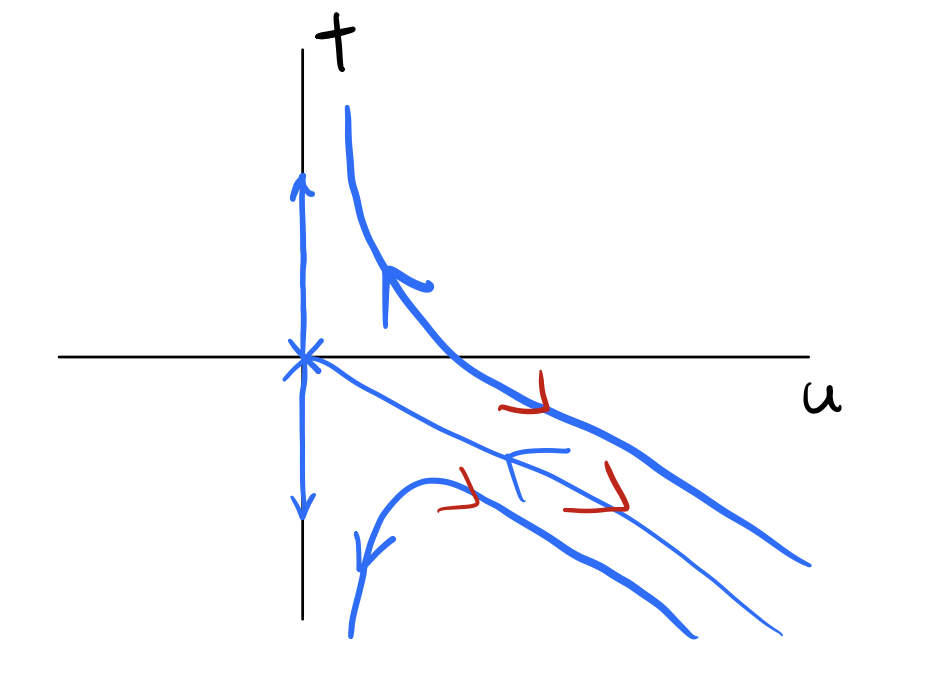
\includegraphics[scale=0.4]{Lectures/Figures/rgflow-linear.png}
    \caption{Flow for linearized RG; for $d > 4$ $u$ flows towards $0$, but for $d < 4$ $u$ diverges to infinity.}
    \label{rgflow-linear}
\end{figure}

There are also second order terms - we will not look at these as there are 36 terms and this will be painful. But we sort of know what to expect. There will be corrections of order $u^2$, so:
\begin{equation}
    \dod{t}{l} = 2 + u(\text{factor}) - Au^2
\end{equation}
\begin{equation}
    \dod{u}{l} = u(4-d) - Bu^2
\end{equation}
Now, if $u$ starts to flow away from the origin, it will get pushed back! In that case, what happens is we get a new critical point at $u^*$, which is equal to:
\begin{equation}
    u^* = \frac{4-d}{B}
\end{equation}
which is where $u$ stops flowing. There will be a corresponding critical value $t^*$:
\begin{equation}
    t^* \sim -Cu^ + \text{(corrections)}
\end{equation}

\begin{figure}[htbp]
    \centering
    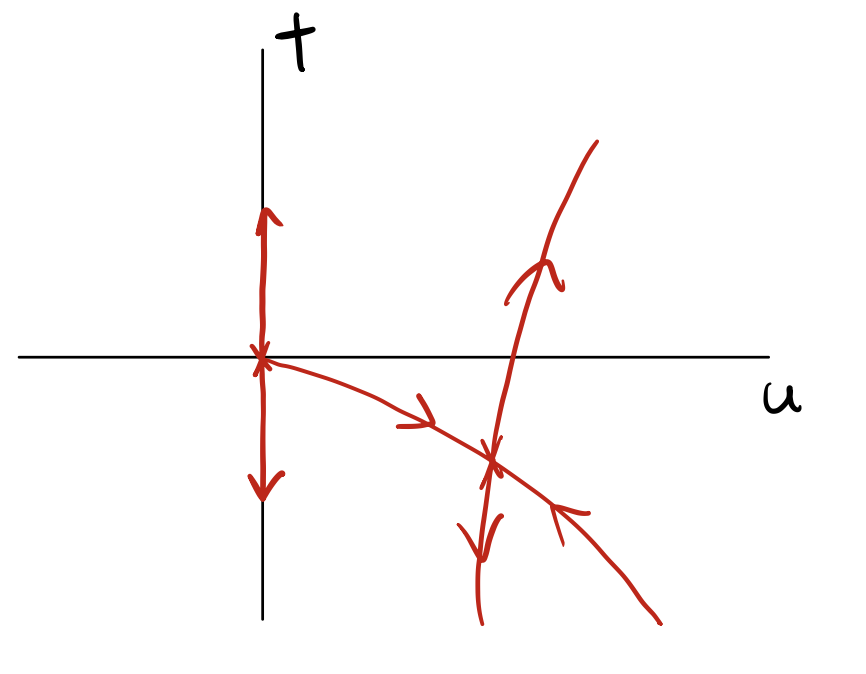
\includegraphics[scale=0.4]{Lectures/Figures/rgflow-quadratic.png}
    \caption{Flow for RG to quadratic order; a new fixed point emerges.}
    \label{rgflow-quadratic}
\end{figure}


This is a rather laborious calcualtion to show this, but it has been done. But what is important to note is that in principle the behaviour is controlled by $4-d$, and if we define $\e = 4-d$, then this is what is known as the $\e$-expansion, i.e. regularizing the problem by working close to a critical dimension:
\begin{equation}
    u^* = \frac{\e}{B}
\end{equation}
The result of which is:
\begin{equation}
    y_t = 2 - \frac{n+2}{n+8}\e + O(\e^2)
\end{equation}
\begin{equation}
    y_u = -\e
\end{equation}
This is a manifestation of universality (I missed why this was...)

One should also check what other kinds of coefficients get generated by this process. If we keep going on, there will be terms of $\e^2$, and we will generate other gradient terms we did not have before. They will always appear one order higher than the previous. At this level, the new fields are generated and are irrelevant at this order.

What happens if we try $\e = 1$ do get $d = 3$? The exponents turn out for Ising model are remarkably close to numerical estimates, even though there is no reason things should have been. We don't know what the radius of convergence of this series is; it is a bit of a punch in the dark. 

Note that the fixed point $(t^*, u^*)$ is the known as the Wilson-Fisher fixed point.

Reviewing exactly what we have done today:
\begin{itemize}
    \item We take a model that has a complicated higher order term, namely the fourth order term.
    \item What we know is that this term can be made small by going into the vicinity of a critical dimension, here $d = 4$. (The scaling dimension of the fourth order term is $4-d$). To the extent that this is a small number, the expansion can be controlled.
    \item Then, we know that the scaling law has to be augmented as we go through perturbatively through terms, with corrections $u, u^2, \ldots$. Therefore the $\dod{t}{l}$ must have the power series functional form that we found. \item The signs of the term we do not necessarily know, but we can guess that we can find solutions by postulating that there exist fixed points of the form as we found.
    \item Then we get a scaling diagram, where in addition to the Gaussian fixed point (unstable in the $u$ direction) we find the Wilson-Fisher fixed point, which $u$ flows to.
    \item Rather than the tedious algebra, the takeaway is the structure of the theory that comes out of it, and what kind of scaling theory it gives us.
\end{itemize}

Next class, we will look at continuous symmetries, which are slightly easier to deal with. We go away from spin waves, towards objects with topology. We shall begin this with the nonlinear-$\sigma$ model (spins of fixed length that can point in any direction). From there, we will go to the 2-D $XY$ model, and start to study topology in spin space.